\section{Cinematica e Dinamica}
La cinematica si occupa della descrizione del moto mentre la dinamica della sua causa. Insieme cinematica e dinamica danno la meccanica.
\definizione{Punto materiale}{Il punto materiale, o particella, è un corpo che presenta dimensioni trascurabili rispetto a quelle dello spazio in cui può muoversi (o degli altri corpi).}{def:puntoMateriale}
Un punto materiale compie solo trasformazioni. Un corpo esteso compie traslazioni e rotazioni e vibrazioni.

Il moto di un punto materiale è determinata se è nota la posizione del punto in funzione del tempo in un dato sistema di riferimento.
\definizione{Traiettoria}{La traiettoria (una curva nello spazio) è il luogo dei punti occupati dal corpo in movimento.}{def:traiettoria}
\definizione{Velocità}{La velocità è la variazione nel tempo della posizione del corpo.}{def:velocità}
\definizione{Accellerazione}{L'acellerazione è variazione nel tempo della velocità.}{def:accellerazione}
\definizione{Moto rettilineo}{Il moto rettilineo si svolge lungo una retta, fissata un'origine e un verso. Il moto cosi è descrivibile secondo un'unica coordinata scalare $x(t)$.}{def:motorett}
\textbf{Diagramma orario} fissa sulle ascisse il tempo $t$ e sulle coordinate la posizone $x$. Rappresenta la posizione lungo la retta del corpo in un determinato istante. (se va avanti o indietro).
\mysubsection{Velocità nel moto rettilineo}
Definiamo la velocità media come il rapporto tra lo spazio e il tempo, tra due punti \[v_m=\frac{\Delta x}{\Delta y}=\frac{x_2-x_1}{t_2-t_1}\]
\definizione{Velocità istantanea}{
La velocità istantanea è la velocità nel moto rettilineo se rendo gli intervalli $\Delta t$ infinitesimali \[\lim\limits_{\Delta t \to 0}\frac{\Delta x}{\Delta y}=\frac{dx}{dt}=v\] La velocità istantanea è la rapidità di variazione della posizione in un dato istante.}{def:velistantanea}
\definizione{Moto rettilineo uniforme}{
Il moto rettilineo uniforme ha $v=v(t)$ costante dato il segno della velocità che indica la direzione del moto.

Nota la legge oraria $x(t)$ tramite derivazione rispetto al tempo è ricavabile la velocità.}{def:defMotoRetUniforme}
\mysubsection{Problema inverso}
Sia un punto materiale in $x$ al tempo $t$ e in $(x+dx)$ al tempo $(t+dt)$. Vale la relazione $dx=v(t)dt$ e avrò \[\Delta x = \int_{x_0}^{x}dx=\int_{t_0}^{t}dt\implies x-x_0=\int_{t_0}^{t}v(t)dt\] da cui ricaviamo la legge oraria $x(t)=x_o+\int_{t_o}^{t}v(t)dt$ e la velocità media $v_m=\frac{1}{t-t_0}\int_{t_0}^{t}v(t)dt$.

Nel moto rettilineo uniforme $v$ è constante e si ottiene \[x(t)=x_0+\int_{t_0}^{t}vdt=x_0+v\int_{t_0}^{t}dt=x_0+v(t-t_0)\] e scegliendo $t_0=0$ si ha $x(t)=x_0+vt$. In questo caso la velocità istantanea coincide con la velocità media.
\definizione{Accelerazione media e istantanea}{L'accellerazione media è la variazione della velocità in una finestra temporale \[a_m=\frac{\Delta v}{\Delta t}\]L'accelerazione istantanea è \[a=\frac{dv}{dt}=\frac{d^2v}{dt^2}\]}{def:accMedia}
Se l'accellerazione è zero siamo nel caso del moto rettilineo uniforme.
\paragraph{Il segno} dell'accellerazione dice se la velocità aumenta o diminuisce nel tempo.
Osservo che il verso del moto è il segno della velocità, non da quello dell'accellerazione.

\paragraph{Problema inverso} \[dv=a(t)dt\implies \Delta v = \int_{v_0}^{v}dv=\int_{t+0}^{t}a(t)dt\]\[v(t)=v_0+\int_{t_0}^{t}a(t)dt\]

Se conosciamo $a(x)$ possiamo fare \[v^2=v_0^2+2\int_{x_0}^{x}a(x)dx\] dato da $a=dv/dt=\frac{dv}{dx}\cdot\frac{dx}{dt}=v\frac{dv}{dx}\implies adx=vdv$.

Nota: $m/s=3.6km/h$.
\definizione{Moto rettilineo uniformemente accelerato}{
\begin{multicols}{2}
	Se l'accellerazione non è costante un moto è definito vario. Un moto con un accellerazione costante è uniformente accelerato, con \[v(t)=v_0+a(t-t_0)\]\[x(t)=x_0+v_0(t-t_0)+1/2a(t-t_0)^2\] ponendo $t_0=0$ si ottiene
	\[\begin{cases}
		v(t)=v_0+at\\
		x(t)=x_0+v_0t+1/2at^2
	\end{cases}\]
	dalla relazione tra velocità e posizione si ottiene \[v^2=v_0^2+2a(x-x_0)\]
\end{multicols}}{motorettuniformacc}
\mysubsection{Caduta verticale die gravi}
Trascurando l'attrito, ogni corpo in caduta libera in prossimità della superfice terrestre si muuove verso il basso con accellerazione costante di modulo $g=0.91m/s^2$.
Fissato l'asse verso l'alto si ha $a=-g$.

Si tratta di un moto uniformemente accellerato con accellerazione identica per tutti i gravi.

\paragraph{Con $v_0=0$} un corpo cade da un'altezza $h$ verso il basso.
\[
\begin{cases}
	v=-gt\\
	x=h-\frac{1}{2}gt^2\\
\end{cases}
\begin{cases}
	v(x)=\sqrt{2g(h-x)}\\
	t(x)=\sqrt{\frac{2(h-x)}{g}}\\
\end{cases}
\]
Condizoni iniziali:$x_0=h, v_0=0, t_0=0$.
Ponendo $x=0$ dal secondo sistema si ottiene:
\subparagraph{Tempo di caduta} $t_c=\sqrt{\frac{2h}{g}}$.
\subparagraph{Velocità al suolo} $v_c=\sqrt{2gh}$.
\paragraph{Con $v_0<0$} un corpo cade da un'altezza $h$ verso il basso.
\[
\begin{cases}
	v=-v_1-gt\\
	x=h-v_1t-\frac{1}{2}gt^2\\
\end{cases}
\begin{cases}
	v(x)=\sqrt{v_1^2+2g(h-x)}\\
	t(x)=-\frac{v_1}{g}+\sqrt{\frac{v_1^2}{g^2}+\frac{2(h-x)}{g}}\\
\end{cases}
\]
Condizioni iniziali: $x_0=h, v_00-v_iv_i>0), t_o=0$. Nota che per $t(x)$ si scarta la soluzione negativa.
Ponendo $x=0$ dal secondo sistema si ottiene:
\subparagraph{Tempo di caduta} $t_c=-\frac{v_1}{g}+\sqrt{\frac{v_1^2}{g^2}\frac{2h}{g}}$.
\subparagraph{Velocità al suolo} $v_c=\sqrt{v_1^2+2gh}$.
\paragraph{Con $v>0$} un corpo lanciato verso l'alto partendo dal suolo.
\[
\begin{cases}
	v = -v_2-gt\\
	x = v_2t-\frac{1}{2}gt^2\\
\end{cases}
\begin{cases}
	v(x)=\pm\sqrt{v_2^2-2g(x)}\\
	t(x)=\frac{v_2}{g}\pm\sqrt{\frac{v_2^2}{g^2}-\frac{2x}{g}}\\
\end{cases}
\]
Condizioni iniziali: $x_0=0, v_0=v_2>0, t_0=0$.
Ponendo $x=0$ dal secondo sistema si ottiene:
\subparagraph{Tempo di caduta} $t_c=\frac{v_2}{g}\pm\frac{v_2}{g}$.
\subparagraph{Velocità al suolo} $v_c=\pm v_2$.
\subparagraph{La leggere oraria} di questo moto è una parabola che interseca l'ascissa in $t=0$ con $v=v_2$ e in $t=\frac{2v_2}{g}$ con $v=-v_2$.

\begin{multicols}{2}
	\noindent Ponendo $v=0$ nella legge oraria troviamo $t_m$, il tempo i corrispondenza della massima altezza raggiunta.\[0=v_2-gt_m\implies t_m=v_2/g\] Il corpo in $t_m$ sta a $x_m=v_2^2/2g$.
	\begin{itemize}
		\item $t<t_m\to v>0$
		\item $t>t_m\to v<0$
		\item $t_{tot}=2t_m$
	\end{itemize}
\end{multicols}
\subsection{Moto del proiettile}
Grave con accellerazione costante di modulo $g$ diretta verso il basso e accellerazione orrizontale nulla.

Preso l'asse $y$ diretto verso l'alto si avrà $a_y=-g, a_x=a_z=0$ all'istante iniziale.

Sia $\vec{v_0}$ la velocità iniziale nel piano $xy$, $v_{0z}=0$ e $v_z=0$ per ogni istante, cosi definità \[\vec{v_0}=v_{0x}\hat{i}+v_{0y}\hat{j}=v_0\cos\Phi_0\hat{i}+v_0\sin\Phi\hat{j}\] Con $\Phi$ l'angolo di lancio rispetto all'origine.
In ogni istante si ha $|\vec{v}|=\sqrt{v_x^2+v_y^2}$ e che $\tan\Phi_0=v_y/v_x$.

Dato $a_x=0$ si ha $v_x(t)=v_0\cos\Phi_0$ e $v_y(t)=v_{y0}+a_yt=v_0\sin\Phi_0-gt$, da cui si ha la legge oraria \[
\begin{cases}
	x(t)=(v_0\cos\Phi_0)t\\
	y(t)=(v_0\sin\Phi_0)t-\frac{1}{2}gt^2\\
\end{cases}
\] Da cui ricaviamo traiettoria e gittata.
\paragraph{La Traiettoria} è parabola passante per il punto di lancio. \[y(x)=(\tan\Phi_0)x-\frac{g}{2v_0^2\cos^2\Phi_0}x^2\]
\paragraph{La Gittata} è la distanza orrizontale totale percorsa. \[R=\frac{v_0^2}{g}\sin2\Phi_0\]


\subsection{Vettori}
\paragraph{Vettore libero} è un'oggetto definito da \textbf{modulo, direzione, verso} che rappresenta uno spostamento indipendente dalla posizione d'applicazione.
\subparagraph{Ugualianza} Due vettori sono uguali solo se hanno tutte e tre le grandezze uguali. Vettori diversi possono avere alcune grandezze uguali.

Se due vettori $\vec{e}, \vec{f}$ differiscono solo per il verso si può dire $\vec{e}=-\vec{f}.$
\paragraph{Vettore applicato} è un vettore con un punto d'applicazione.
\paragraph{Prodotto con scalare} Dati $\vec{a}$ vettore e $m$ scalare ho \[\vec{b}=m\vec{a}\]In cui la direzione è mantenuta, il modulo è $m$ volte il modulo di $\vec{a}$ e il verso è lo stesso se $m>0$, altrimenti è l'opposto.
\paragraph{Versore} è un vettore di modulo unitario, $|\vec{u}|=1$. Tutti i vettori con stessa direzione e verso a $\vec{u}$ sono scrivibili come $\vec{a}=a\vec{u}$, dove $a$ specifica il modulo e verso mentre $\vec{u}$ la direzione.
Notazionalmente un versore si indica $\hat{u}_r$.

Dato un vettore $\vec{a}$ posso ottenerne il versore con $\frac{\vec{a}}{|\vec{a}|}=\hat{u}_a$.
\paragraph{La Somma} di vettori è commutativa, associativa e graficamente si ottiene mettendo un vettore in coda all'altro. \[\vec{c}=\vec{a}+\vec{b}\]
\subparagraph{Vettori paralleli} si sommano i moduli con segno determinato dal verso. \[\vec{a_1}+\vec{a_2}=(a_1+a_2)\hat{u}\]
\paragraph{La Differenza} di vettori è la somma di uno con l'opposto dell'altro. \[\vec{a}-\vec{b}=\vec{a}+(-\vec{b})\]
\paragraph{Scomposizione} Dato $\vec{v}$ e due direzioni orientate $r, s$ posso scrivere \[\vec{v}=\vec{v}_r+\vec{v}_s=v_r\hat{r}+v_s\hat{s}\] Dove $\vec{v}_r, \vec{v}_s$ sono i vettori componenti lungo $r,s$ e $\hat{r}, \hat{s}$ sono i versori che definiscono direzione e verso lungo $r,s$.

La scomposizione può essere anche in più direzioni. La somma di vettori scomposisti è la somma dei coefficenti.
\paragraph{Prodotto scalare} Dati $\vec{a}, \vec{b}$ e $\theta$ l'angolo formato dai due vettori ottengo il prodotto scalare con \[\vec{a}\cdot\vec{b}=ab\cos(\theta)\] Graficamente è una proiezione ortogonale.
\subparagraph{Proprietà}
\begin{itemize}
	\item Il prodotto è nullo se uno dei vettori è nullo o $\theta=90°$.
	\item Il prodotto è commutativo, distributivo e gli scalari possono essere spostati.
	\item Se i due vettori sono uguali si ha $a^2$.
	\item Non è iterabile.
\end{itemize}
\paragraph{Prodotto vettoriale} tra due vettori $\vec{a}, \vec{b}$ è un vettore $\vec{c}$ \[\vec{c}=\vec{a}\times\vec{b}\] La direzione di $\vec{c}$ è perpendicolare al piano $\vec{a}, \vec{b}$, il verso è destrorso rispetto alla rotazione $\vec{a}\to\vec{b}$ e il modulo è $c=ab\sin(\theta)$ con $0\leqslant \theta \leqslant \pi$.
\subparagraph{Proprietà}
\begin{itemize}
	\item $\vec{a}\times\vec{a}=\vec{a}\times\lambda\vec{a}=0$.
	\item Anticommutativa: $\vec{a}\times\vec{b}=-\vec{b}\times\vec{a}$.
	\item Distributiva: $\vec{a}\times(\vec{b}+\vec{c})=\vec{a}\times\vec{b}+\vec{a}\times\vec{c}$.
	\item $\vec{a}\times(\lambda\vec{b})=\lambda(\vec{a}\times\vec{b})$.
	\item Non vale la proprietà associativa.
\end{itemize}

\subsection{Moto Circolare}
Dato un sistema di riferimento con origine nel centro della traiettoria circolare e piano $xy$ nel piano della circonferenza.
\begin{multicols}{2}
	\begin{figure}[H]
		\centering
		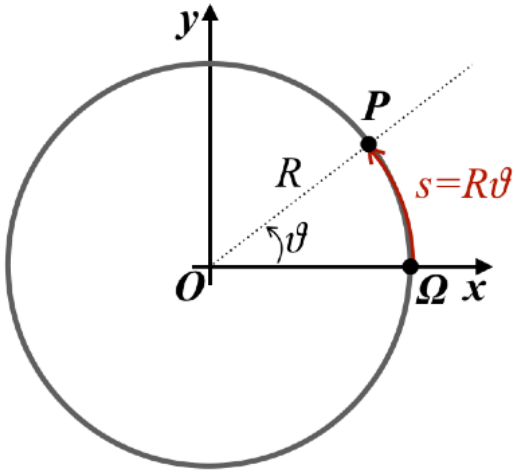
\includegraphics[width=0.6\linewidth]{img/motocircolare.png}
	\end{figure}
	\[
	\begin{cases}
		x = R\cos\Theta\\
		y = R\sin\Theta\\
		z = 0\\
	\end{cases}
	\]
	Vetotre poszione: \[\vec{r}=R\cos\theta\hat{i}+R\sin\theta\hat{j}\]
	In $\Omega=(R, 0 0)$ si ha origine della ascissa curvilinea di rotazione antioraria, $s=R\theta0(0\leqslant s \leqslant 2\pi R)$, ossia la distanza percorsa lungo la circonferenza da $\Omega$ fino $P$. \[\theta=s/R\]
\end{multicols}
\paragraph{Moto circolare uniforme} ha la velocità scalare $v_s$ costante. \[v_s=R\omega\] Con $w=\frac{v_s}{R}$ la velocità angolare.

Legge oraria dell'angolo $\theta$: $\theta(t)=\theta_0+\omega(t-t_0)$.

Se si pone $t_0=0$ e $\theta(t)=\omega t$ si ha $\theta(t)=\omega t$.
\subparagraph{Accellerazione centripeda} Dati
\[
\begin{cases}
	\vec{r}(t)=R\cos(\omega t)\hat{i}+R\sin(\omega t)\hat{j}\\
	\vec{v}(t)=-\omega R \sin(\omega t)\hat{i}+\omega R \cos(\omega t)\hat{j}\\
	\vec{a}(t)=-\omega^2\vec{r}(t)\\
\end{cases}
\]
Sappiamo che l'accellerazione è diversa da 0, è centripeda e costante in modulo. $\vec(a), \vec{r}$ hanno stessa direzione e verso opposto dando un vettore che da $P$ va a $O$. \[a_c=|\vec{a}(t)|=\omega^2R=\frac{v_s^2}{R}\]
Costante in modulo e proporzionale alla velocità angolare.
\paragraph{Accellerazione tangenziale} quando il moto circolare non uniforme, con velocità scalare e angolare non costanti, si ha velocità centripeda e tangenziale.

La velocità totale è somma vettoriale delle velocità perpendicolari centripeda e tangenziale.

accellerazione angolare $\alpha=d\omega/dt$, tangenziale $a_t=\alpha R$ e totale $a=R\sqrt{\omega^4+\alpha^2}$